\documentclass[thesis]{subfiles}

\begin{document}

\OnlyInSubfile{\appendix}
\chapter{Chemfiles: library for chemistry Input/Output}
\label{sec:chemfiles}

\vfill
\begin{center}
    
\includegraphics[width=.3\textwidth]{figures/images/chemfiles-logo}
\end{center}
\vfill

During my PhD, I also wrote chemfiles, a library that allow to read and write
multiple file formats used in computational chemistry. I will present here the
software, its goals and some implementation strategy I used.

\newpage
\section{The computational chemistry formats zoo}

A recurrent pain point for anyone working in the theoretical and computational
chemistry field is the multiplication of file formats. Every simulation software
comes with its own set of files formats. And it is up to the user to adapt, and
learn how to work with the set of formats used by a specific software.

These formats are used to store data generated by a simulation software, before
analyzing it either through visualization of the atoms and their individual
motions; or by computing properties of the system from the positions and
velocities, using the framework of statistical thermodynamics presented in
section~\ref{sec:statistical-thermo}.

At the same time, every format contains the same kind of information: atomic
names, positions, velocities, forces, and topological information (bonds,
residues, \etc). Different formats exist because in addition to storing this
basic data, they have different use cases. For example, the XYZ format is very
simple to read an write, both by hand and when creating new softwares. Binary
formats, such as NetCDF or TNG allow to store huge trajectories efficiently,
both in term of disk size and reading speed. The PBD, mmCIF and MMTF format are
optimized to store proteins and other bio-molecules.

\begin{figure}[ht]
    \centering
    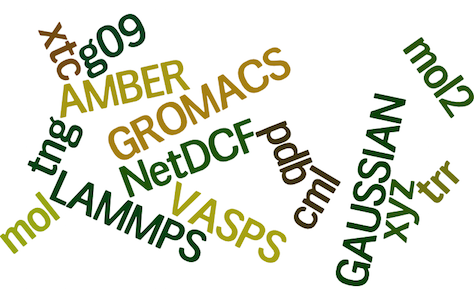
\includegraphics[width=.4\textwidth]{figures/images/files-formats}
    \caption{Some of the existing formats used in computational chemistry.}
    \label{fig:chemfiles:formats}
\end{figure}

This multiplication of formats means that there is less interoperability between
different software. Analysis and visualization software support specific

To run analysis on the results of a simulation wee have to
either use readily available algorithms, or learn how to read the format of our
current software. There is quite a lot of friction to switch between simulation
softwares or to use a specific analysis code

Chemfiles is an attempt to provide an unified and simple interface for
programmers to work with all these file formats. In order to do so, it defines a
representation for the data that can exist in various formats, and transparently
reads and writes files from and to this representation. Which means that
software developers only need to learn how to use chemfiles, and can then use it
to read or write every supported file format!

Chemfiles is a software library; a collection of functions and classes meant to
be integrated into other software. It can be used in simulation software (for
example Domino uses chemfiles for reading the initial configuration and writing
the trajectory); visualization or analysis software, such as cfiles, presented
below.

\section{Goals and missions}

\subsection{Chemfiles goals and non-goals}

The main goal of chemfiles is to be useful to the research community at large.
To be useful, chemfiles must first be usable, and different researchers and
softwares developers work with different computing environments. Chemfiles is
portable between different platforms, operating systems (Windows, GNU/Linux,
macOS), word sizes (32 or 64-bits environments) and CPU architecture (Intel,
ARM, PowerPC, \dots). It is also usable from multiple language, to allow any
computation chemistry project to use it, regardless of the implementation
language the authors choose. The core of the library is written in \cxx, and it
offers interfaces to C, Python, Fortran, Julia and Rust.

Computational chemistry is used with a wide range of systems, and each kind of
system has specific requirements, which chemfiles tries to support. For
example, simulations of bio-molecules such as proteins or nucleic acid strands
uses complex topologies, grouping some atoms in residues or monomers.
Oftentimes, this topology is stored in a separated file. While bio-molecules
simulation mostly only needs orthorhombic unit cells, material science and
crystallographic data needs to describe triclinic unit cells, where some of the
angles are not 90°. Finally, when working with simulations in the grand
canonical ensemble such as GCMC, the number of atoms in the system changes along
the trajectory. Support for such simulations where the number of atoms is not
constant is often missing from existing software.

Chemfiles also has explicit non-goals: features that should not be part of
chemfiles itself, but could instead be built on the top of it. For example,
trajectory analysis, energy minimization or simulation algorithms would add to
much complexity to the code. Chemfiles is also actively trying \textbf{not} to
create a new format. Instead, it focuses on providing interoperability between
existing formats.

\subsection{Existing alternatives}

Multiple attempts to solve the issue of file format multiplication already
exist. Here, I will review some of these, and compare them to chemfiles,
given the goals stated above for this kind of library.

\subsubsection{OpenBabel}

OpenBabel\cite{OBoyle2011} is \cxx library that provides read and write
capabilities to other softwares. It is a well established software supporting
more than 110 different file formats. Unfortunely, it only support text/ASCII
based formats, and no binary formats such as Amber NetCDF or Gromacs TNG. Such
binary formats are used to store big trajectories, are faster and take less
space than equivalent text formats.

Two other caveats of OpenBabel for me were the complexity of the programming
interface, and its license. OpenBabel is distributed under the Gnu Public
License (GPL), which makes it harder to use in projects which do not also use
the GPL license. Concerning the programming interface, OpenBabel is written with
the \cxx 98 standard, and a lot of member functions return raw pointers to
internal data directly, instead of the more modern references or smart pointers.

This type of API \TODO

\subsubsection{Other alternatives}

\begin{table}[ht]
    \centering
    \caption{Summary of existing software library providing read/write capabilities.}
    \label{tab:chemfiles:alternatives}
    \def\nope{\textcolor{red}{\Large$\circleddash$}}
    \def\yep{\textcolor{webgreen}{\Large$\oplus$}}
    \begin{tabularx}{0.8\textwidth}{X c c c c}
        \toprule
            \bfseries Project            & language & \cxx compatible & GCMC  & license \\
        \midrule
            OpenBabel\cite{OBoyle2011}   &   \cxx   &      \yep       & \nope & GPL-2   \\
            VMD\cite{Humphrey1996}       &  C/\cxx  &      \yep       & \nope & BSD     \\
            MDAnalysis\cite{Michaud2011} &  Python  &      \nope      & \nope & GPL-2   \\
            cclib\cite{OBoyle2008}       &  Python  &      \nope      & \nope & BSD     \\
            ASE\cite{HjorthLarsen2017}   &  Python  &      \nope      & \nope & LGPL    \\
            CDK\cite{Willighagen2017}    &  Java    &      \nope      & \nope & LGPL    \\
        \bottomrule
    \end{tabularx}
\end{table}

\subsection{Some code statistics}

I started working on chemfiles in December 2014, and released the 0.1 version
the 16th of May 2015. Since then, I released 8 new versions, the last one being
version 0.9, which was released on the 31 of March 2019. During this period,
they have been 1500 modifications (taken as git commits) in the core \cxx
chemfiles library, leading to a library containing 23 000 lines of code, as well
as 11 000 lines of test code. Bindings to chemfiles in other languages (Python,
Fortran, Rust, Julia) contains 800 commits, 12 000 lines of code, and 5 000
lines of tests.

A few people helped me making chemfiles what it is, I would like to thank here
again Jonathan Fine from Purdue University (USA); Patricio Germán Barletta from
Universidad Nacional de Quilmes (Argentina); Laura Scalfi and Elsa Perrin from
École Normale Supérieure (France).

\section{Architecture overview}

...

\subsection{Implemented formats}

\section{Storing additional data: properties}

=> dynamically typed

\section{Atomic selection language}

\subsection{Multi-atoms selections}

\subsection{Implementation strategy}

\section{Using a library from multiple programming languages}

\section{cfiles: analysis of trajectories}

\subsection{Algorithm for fast auto-correlations}

\subsection{Elastic constants from fluctuations}

\OnlyInSubfile{\printbibliography}

\end{document}
